%!TEX root = ../main.tex
\section{Design} \label{sec:design}

This chapter will set focus on the research from the analysis to create a blueprint of our desired product that will fulfill the demands from our list of requirements. The prototype is going to be split into three different parts.

\begin{itemize}
\item Pacman
\item Simulation
\item Genetic Algorithm
\end{itemize}

The prototype should work as following:

New modes for the ghosts will be created that can be controlled by a finite state machine. This will create a mode cycle that will be able to be manipulated by a genetic algorithm. The goal is then to create a simulation system that can create simulations with new data sets for a fitness function to evaluate in the genetic algorithm. Then return the mode cycle that match the player’s performance for next game of pacman (See Fig. Design Plan).


\begin{figure}[!htbp]
\centering
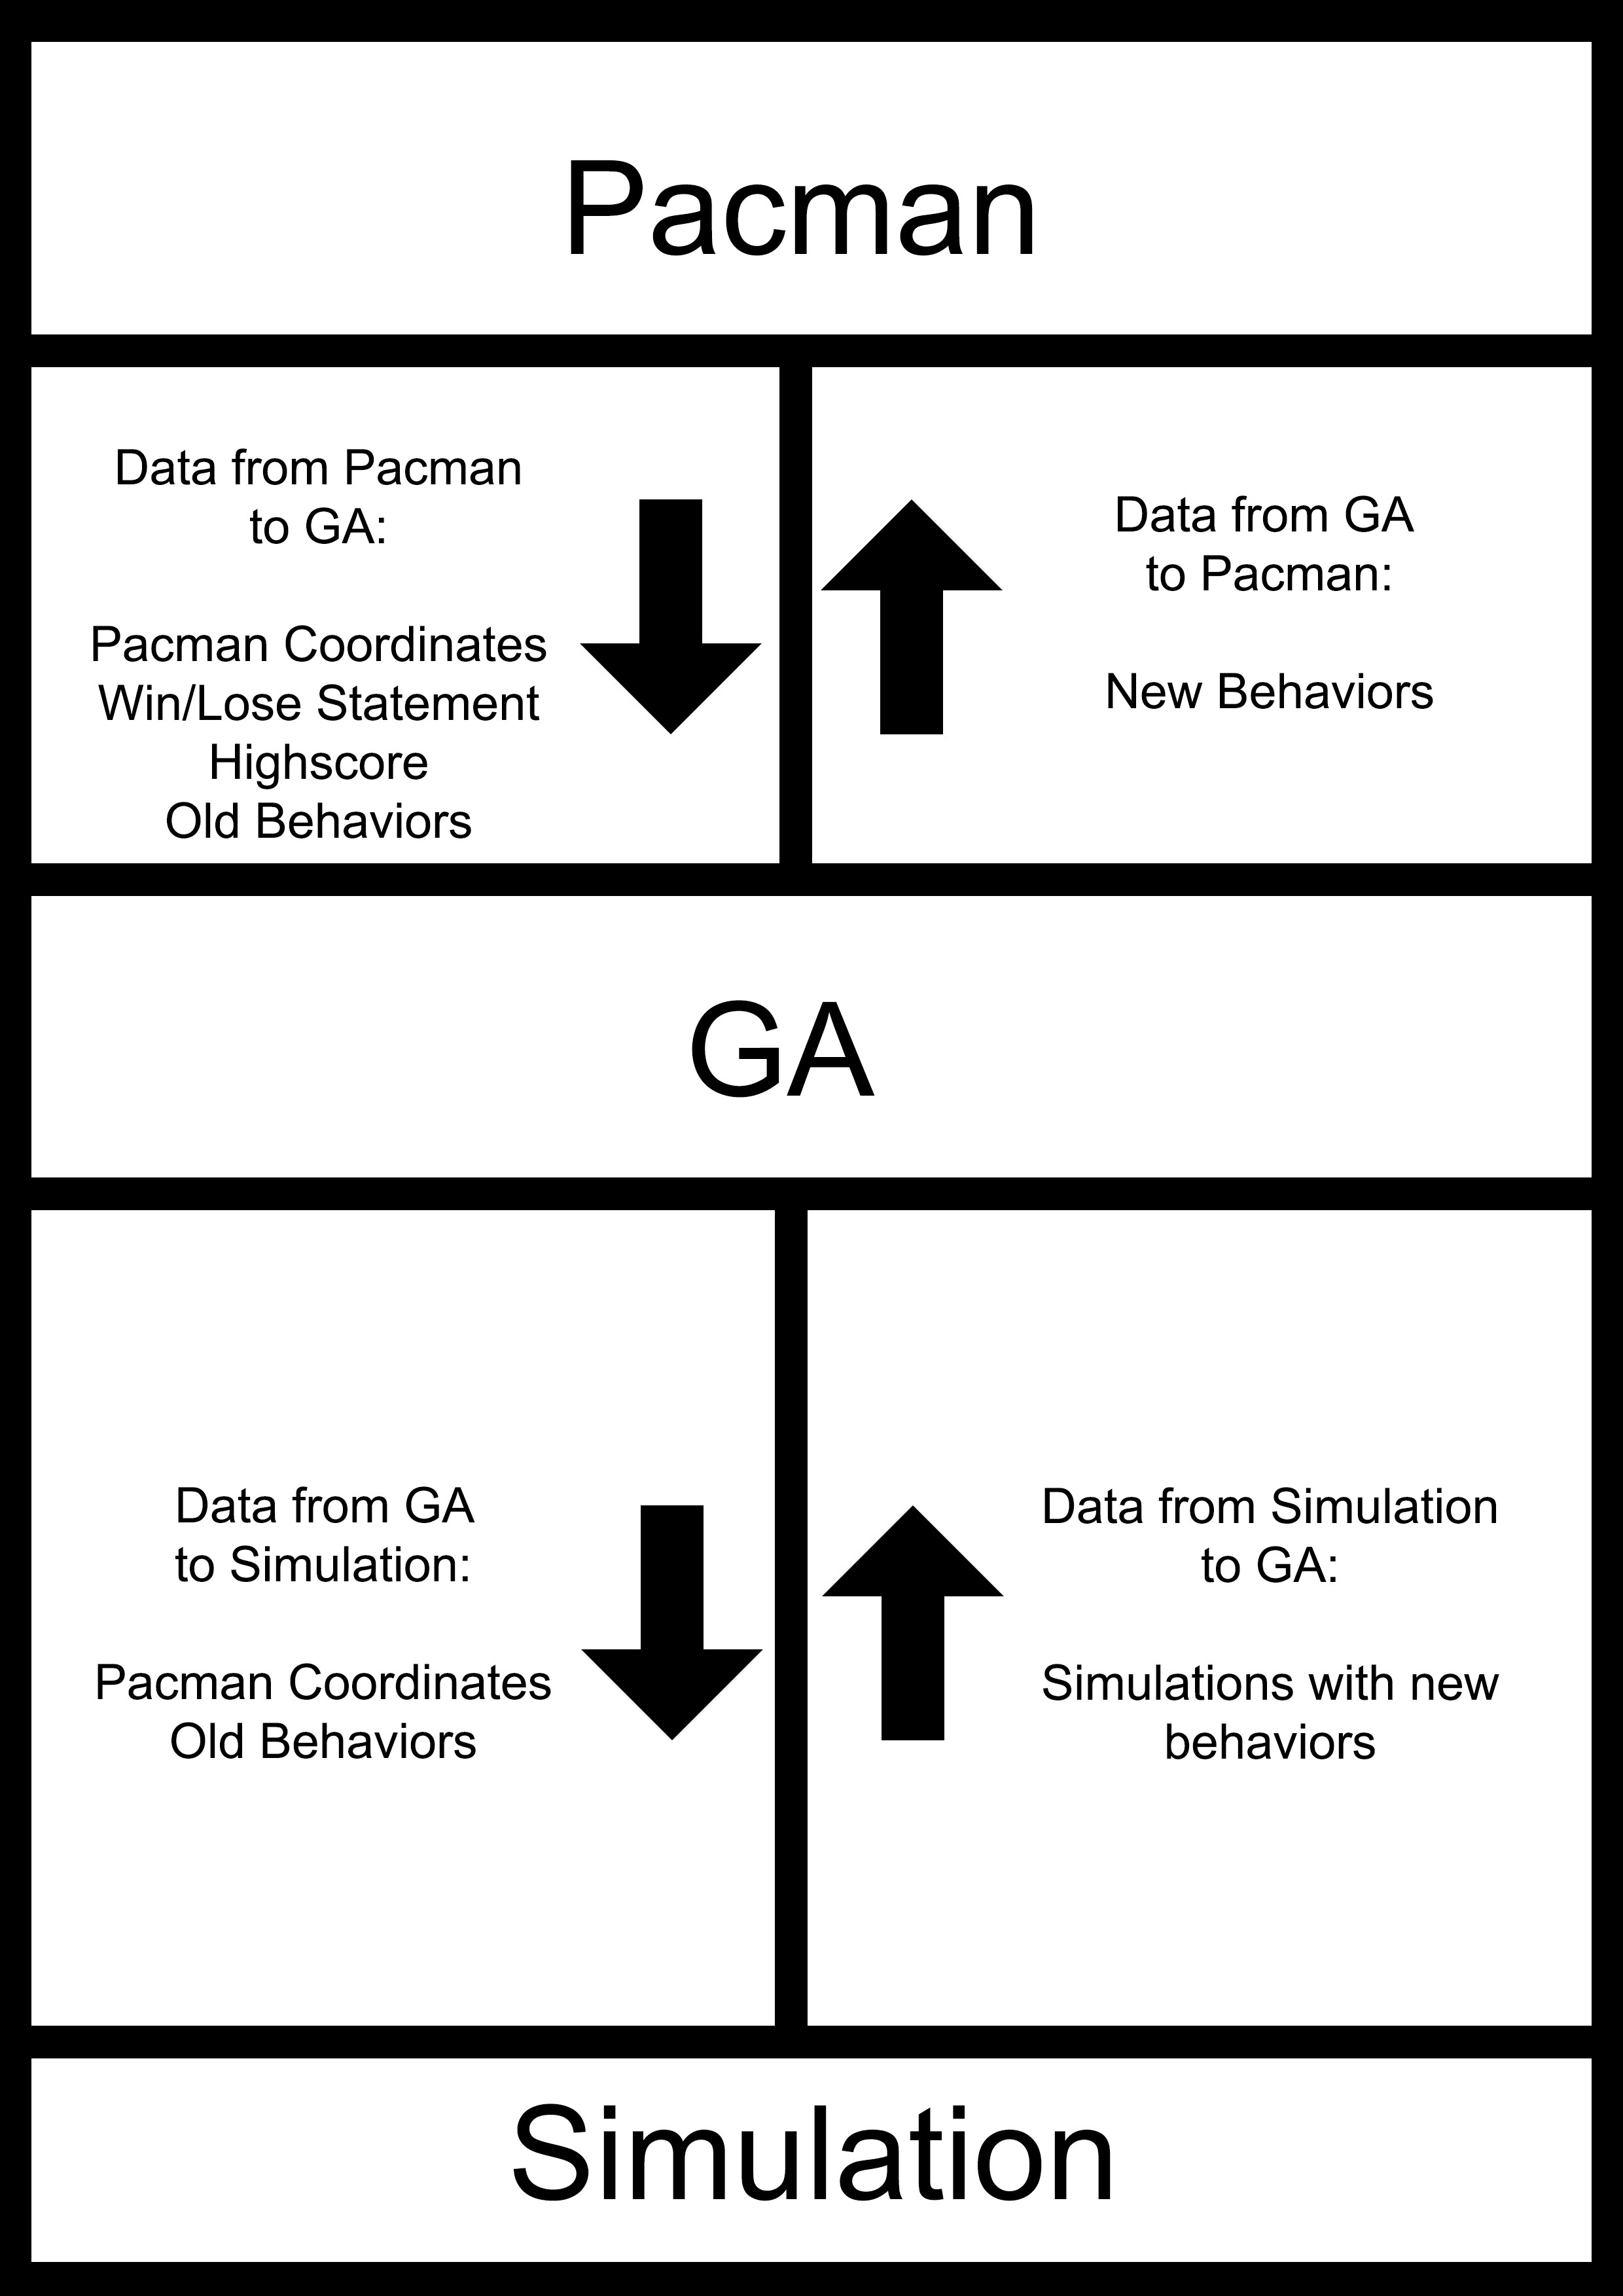
\includegraphics[width=0.5\textwidth]{D1.png}
\caption{ Design Plan }
\label{fig:DesignPlan}
\end{figure}

\subsection{Pacman Modes}\label{ssec:design_modes}

The original Pacman \ref{ssec:pacmandetail} in its current state is not optimized for the use of a genetic algorithm. That is why it has to be tailored into a finite state machine that can be linked with the genetic algorithm and change the values that is being sent as input. We want to base this finite state machine on the different ghost modes \ref{ssec:ai_behavior}. That means the modes are going to be switched during the gameplay and by that each ghost will no longer have a specific role in the game. An example could be that a ghost would change mode every 10 seconds or every 1000 frames and activate either chase, scatter or random. Each ghosts would then have their own chance of activating the different modes, an example could be a more aggressive ghost with high chase value like this:



\begin{center}
Ghost:
Chase - 60\%
Scatter - 30\%
Idle - 10\%
\end{center}


The point system is based on the original pacman. Each dot will grant points which will make sure that you will have a minimum score if completing the level. The energizers won’t directly give you points, in order to obtain points in energized mode the ghosts has to be eaten by pacman. Fruits will spawn around the level and grant a small amount of points. If the player wants to increase the amount of points for the level the player has to fulfill these objectives. All of these points will be used in the evaluation score.


The new modes will be as follows:

\subsubsection{Chase}
The chase-mode will be based on Blinky (\ref{ssec:ai_behavior}) from the original pacman. It will be modified in a few ways to make it more optimal and adjust it so it will not make problems with the new mode cycle. An A* (A-Star) Pathfinder will be used as a pathfinding method. It is a search algorithm which always tracks the fastest way to pacman by the use of calculating coordinates (also known as Nodes) from the ghost and towards its destination. The Elroy mode(\ref{ssec:ai_behavior}) will be removed since it adds an additional difficulty factor with the increased speed of the ghost. It would also create complications with the new mode cycle system, if chase-mode was engaged and all other modes were to be ignored.


\begin{figure}[!htbp]
\centering
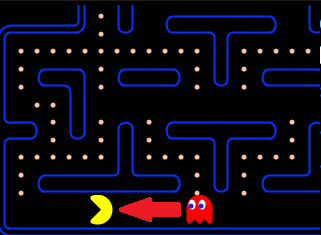
\includegraphics[scale=0.5]{D2.png}
\caption{ Chase Function }
\label{fig:Chase}
\end{figure}


\subsubsection{Scatter}
The scatter-mode will act as in the original pacman. The only change will be that it also would use the new A* Pathfinding system to find the corner that the ghost belongs to and create a patrol path that the ghost will follow.


\begin{figure}[!htbp]
\centering
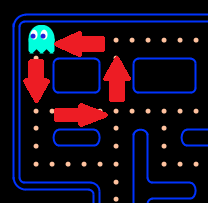
\includegraphics[scale=0.5]{D3.png}
\caption{ Scatter Function }
\label{fig:Scatter}
\end{figure}


\subsubsection{Random and Frightened}
The random and frightened mode will both use the same movement system. When a ghost meets an intersection in the maze it will then make a random decision about which way to go. Obviously the ghost won’t be allowed to move back in the direction which it came. In frightened mode the ghost keeps the same system but will also keep in mind where in the maze pacman is located and try to avoid going in direction which pacman is located.


\begin{figure}[!htbp]
\centering
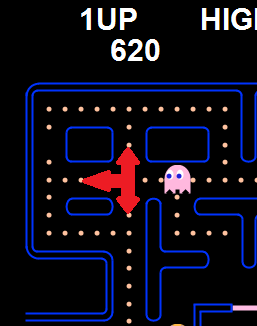
\includegraphics[scale=0.5]{D4.png}
\caption{ Random Function }
\label{fig:Random}
\end{figure}

\begin{figure}[!htbp]
\centering
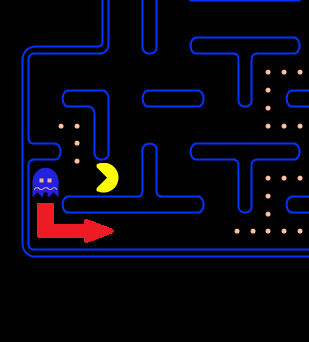
\includegraphics[scale=0.5]{D5.png}
\caption{ Frightened Function }
\label{fig:Frightened}
\end{figure}

\subsubsection{A* Pathfinder}
As mentioned before an A* Pathfinder (\autocite{Boris}) will be the pathfinder choice, this will replace the calculation the ghosts make each intersection in the maze and replace it with a system that always tracks the fastest way to pacman.

The A* Pathfinder work as following:

As seen on A* Fig (1) a grid is applied over the game maze. Since the original pacman also is a grid based game this implementation will be good match for the game. The grid is informed about which coordinates that are able to be used as a path. These coordinates will be marked as true, and the rest, which in our case are walls, will be marked as false. A start point, in our case the ghost, and an end point which is pacman is being placed on the grid.


\begin{figure}[!htbp]
\centering
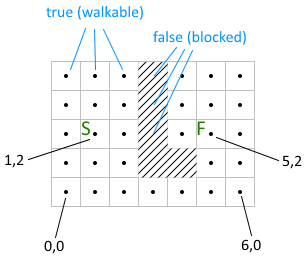
\includegraphics[scale=0.5]{D6.png}
\caption{ A* Part 1 }
\label{fig:A1}
\end{figure}

Every point in the grid has been giving three values which is F , G and H as seen in A* Fig (2). In this case a node is a set of coordinates.

G is the length of the path from the start node to the current point.
H is the distance from the current node and until the end point.
F is the total length of the route which it both the G and H added together.


\begin{figure}[!htbp]
\centering
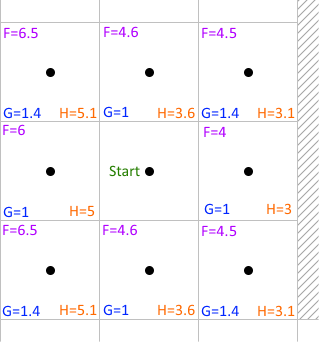
\includegraphics[scale=0.5]{D7.png}
\caption{  A* Part 2 }
\label{fig:A2}
\end{figure}


With these values given to the nodes the system is now ready to calculate the most optimal route to take. The system will value the nodes and put them in a list so they can be evaluated. The node with the lowest H value to be the fastest way to the end point. After a step is taken the node is being set as closed as can be seen on A* Fig (3) in order to make sure that the system won’t use the same node again.


\begin{figure}[!htbp]
\centering
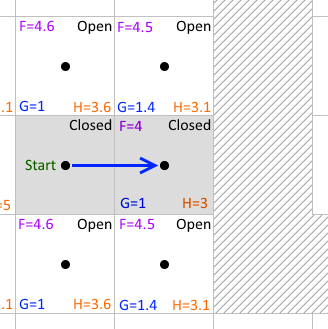
\includegraphics[scale=0.5]{D8.png}
\caption{  A* Part 3 }
\label{fig:A3}
\end{figure}


Another step in the process is to make sure the system also can calculate and find the fastest way through a diagonal path. In our case it won’t be needed since there is no diagonal paths to take in pacman.


\begin{figure}[!htbp]
\centering
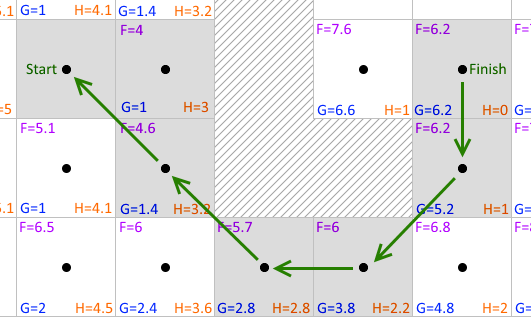
\includegraphics[scale=0.5]{D9.png}
\caption{  A* Part 4 }
\label{fig:A4}
\end{figure}


\subsubsection{Simulation}

Now that the game has its modes; mode cycle and pathfinding adapted to the genetic algorithm, it needs a way to send these informations into the system. A method could be a simulation that can simulate games based on information from a level completed by a player. During a game of pacman the coordinates of the players movements could be recorded and put into an array with timestamps that later can be played in the simulation and simulate the exact movements from the last game. The speed could then be increased to run faster simulations and by that increase the rate of information the genetic algorithm can receive. The information received by the genetic algorithm will be the simulation high score that can be used in the fitness function to calculate the most optimal simulation.


\subsection{Genetic Algorithm}

The information the GA receives is the players high-score and win/lose condition from the last played game. Our GA will be based on the research found in the analysis but before the algorithm is functional the GA variables (section \ref{sec:lor}) from the list of requirements has to be fulfilled.


\subsubsection{Chromosomes}

Each chromosome serves as a single solution and in our case we want to find a way to optimize the modes for our ghosts. So each solution should contain a set of four genes of different sets of modes that combined should be able to make the game more challenging for the player playing with ghosts that has the next generation modes.

\subsubsection{Population Size}

The population size is based on the amount of simulation that our system can provide. According to our initial research (section \ref{ssec:ga}) a good population size is about 100. That means between the first generation and the second generation an amount of 100 simulations has to be played and analyzed before the next game of pacman can take place.


\subsubsection{Fitness function and Fitness Score}

The fitness function is going to be based on the simulation high scores. After the simulations has been played each simulation has been given a high score of how well pacman did in the current round. If pacman/player dies with a low highscore, it means that the ghosts have been very

successful and that chromosome then gets a high fitness score The simulations will be compared and the simulation that gave pacman the lowest high score will be the winner of that current generation.


\subsubsection{Selection}

Elitism
We are looking for a selection method that increases fast and keeps the best solutions and improves them. According to our research (section \ref{ssec:ga}) Elitism fulfill our requirements and priorities like this, Elitism always uses the best chromosomes or the single best according to what the setup is. This will increase the performance of the genetic algorithm rapidly.

\subsubsection{Crossover}
The crossover is based on our research and is being set to 80%

Single Point Crossover \cite{MarekOkbitko1998}:
This method works by taking one small part of a chromosome A and swaps that into chromosome B and by that create a changed chromosome that can be tested once again (See fig. 1).


\begin{figure}[!htbp]
\centering
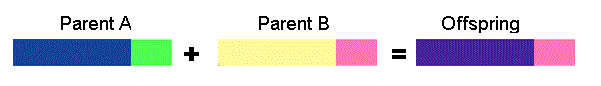
\includegraphics[scale=0.5]{D11.png}
\caption{ Single Point Crossover }
\label{fig:Crossover}
\end{figure}


\subsubsection{Mutation}
As mutation is there to create small random changes in the genes we want it to be low. This is the case since we want our chromosomes to be based on the simulations and not entirely by random mutations. We follow the recommendations from our research (section \ref{ssec:ga}) and place the mutation rate as 0.5%.

\subsection{UML}

\begin{figure}[!htbp]
\centering
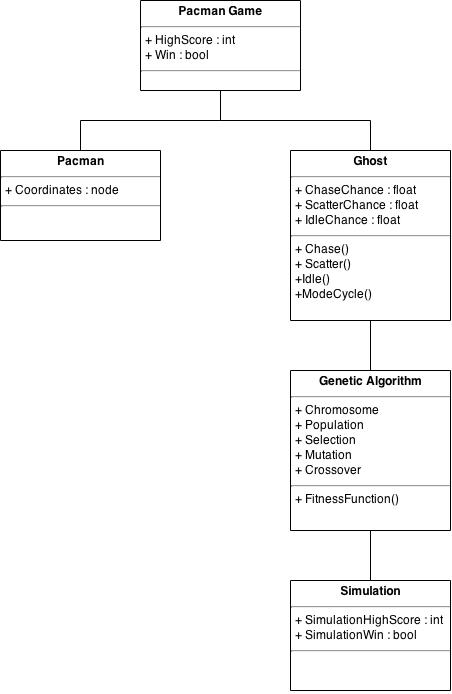
\includegraphics[scale=0.5]{D12.jpg}
\caption{ UML }
\label{fig:UML}
\end{figure}

\subsection{Summary}

The prototype should work as following:

\begin{enumerate}
\item A player plays a level of Pacman.

After the playthrough of the pacman level af set of coordinates of pacman is saved in an array and ready for the simulation to use.

\item The genetic algorithm creates new mode cycles that will be simulated

Based on the first generation chromosome the genetic algorithm will create new chromosomes that will be used in the new population.

\item The simulations use the player coordinates as input for simulating.

An amount of simulations is being played based on the population size and will generate a set of data for the fitness function to evaluate.

\item The simulations will be evaluated and the winning chromosome will be returned to the Pacman game.

\item The player will play a game with the new generation of ghost modes that should match the players performance.

\end{enumerate}

